\documentclass[a4paper,12pt]{article}
\usepackage[polish]{babel}
\usepackage[utf8]{inputenc}
\usepackage{amsfonts}
\usepackage{indentfirst}
\usepackage[T1]{fontenc}
\usepackage{amsmath}
\usepackage{hyperref}
\usepackage{graphicx}
\usepackage{subfig}
\usepackage{fancyvrb}
\usepackage{wrapfig}
\usepackage[toc,page]{appendix} % for appendix

\textwidth\paperwidth
\advance\textwidth -45mm
\oddsidemargin 18mm
\advance\oddsidemargin -18mm
\evensidemargin 18mm
\advance\evensidemargin -18mm
\topmargin -30mm
\advance\topmargin 17mm
\setlength\textheight{45\baselineskip}
\addtolength\textheight{\topskip}
\marginparwidth 15mm

\addto\captionspolish{ % rename Appendices title to Dodatki
\renewcommand\appendixname{Dodatek}
\renewcommand\appendixpagename{Dodatki}
}


\title{
Zaawansowane metody uczenia maszynowego \\
Projekt 1
}
\author{
Mikołaj Małkiński \\
\texttt{malkinskim@student.mini.pw.edu.pl}
}
\date{\today}

\begin{document}
    \maketitle

    \section{Przygotowanie danych}

    \subsection{Brakujące dane}
    Zbiór danych zawiera wiele kolumn które nie są w pełni wypełnione danymi.
    Analiza wykazała, że tylko 20 kolumn posiadały wszystkie wartości.
    Rysunek~\ref{fig:missing-data} przedstawia zależność między stopniem braku danych a liczbą kolumn.
    Istnieje kilka możliwych podejść które można zastosować w tym przypadku.
    Po pierwsze, można kompletnie zignorować i wybrać model który jest w stanie sam odpowiednio obsłużyć luki w zbiorze.
    Przykładem takiego modelu jest \textit{XGBoost}.
    Jednakże, nie wszystkie algorytmy do klasyfikacji są przygotowane na braki w danych,
    Dlatego, aby móc porównać działanie kilku modeli na tym samym zbiorze podjęto decyzję o wypełnieniu brakujących danych.

    \begin{wrapfigure}{r}{0.5\linewidth}
        \centering
        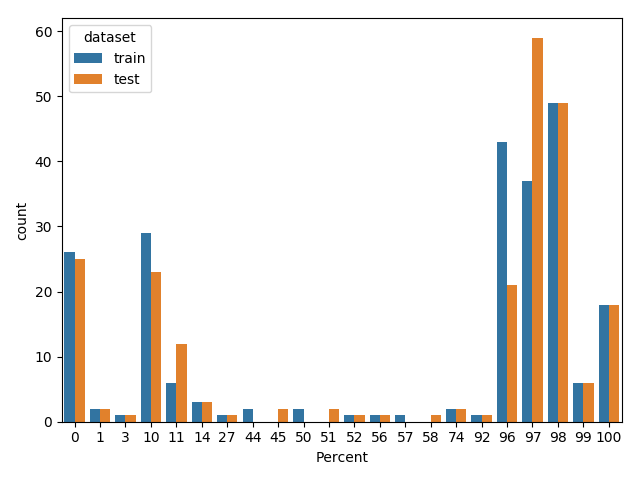
\includegraphics[width=\linewidth]{../images/missing-data.png}
        \caption{Liczba kolumn posiadających dany procent brakujących danych z podziałem na zbiór treningowy i testowy}
        \label{fig:missing-data}
    \end{wrapfigure}

    Niektóre z kolumn posiadały nawet ponad 90\% brakująych danych.
    Nie mając żadnych informacji o zbiorze danych oraz nie wiedząc co dana kolumna reprezentuje, ciężko stwierdzić z czego wynika taki duży brak.
    Może to oznaczać zwyczajnie brak pomiaru, wartość ważną równie dobrze jak ta która istnieje w danej kolumnie lub w danym przypadku wartość w tej kolumnie może nie mieć żadnego znaczenia dla konkretnego wiersza.
    Ze względu na duży rozmiar zbioru danych, podjęto decyzję o kompletnym usunięciu części z takich kolumn, które mają więcej braków niż 90\%.
    Resztę poddano imputacji.

    Kolumny w zbiorze można podzielić na 2 rodzaje: \textit{numeryczne} i \textit{kategoryczne}.
    Aby wypełnić pierwsze z nich, brakujące dane w każdej kolumnie wypełniono jej medianą.
    Oczywiście w innych przypadkach mogłyby zostać użyte także inne funkcje, takie jak średnia lub moda.
    W przypadku kolumn kategorycznych, dodano nową kategorię: \textit{unknown}, która wypełniła braki w tych kolumnach.

    \subsection{Unikalność danych}
    Następnie, analizie poddano liczbę unikalnych wartości dla każdej z kolumn.
    Zbiór zawierał kolumny wypełnione tylko jedną tą samą wartością.
    Takie kolumny nie niosą ze sobą żadnej wartości więc zostały one usunięte
    Dodatkowo, część kolumn kategorycznych, posiadały bardzo dużo unikalnych wartości.
    Można przypuszczać że są to dane tekstowe, które także nie przyniosą pozytywnych efektów w klasyfikacji.
    Dlatego, kolumny mające więcej niż 100 unikalnych wartości zostały usunięte.

    \subsection{Kolumny kategoryczne}
    Niektóre algorytmy klasyfikacji wymagają aby zbiory na których zostaną użyte posiadały tylko cechy numeryczne.
    Z tego powodu, cechy kategoryczne musiały zostać przekształcone w liczbowe.
    Najprostszym sposobem jest zamienienie każdej z kategorii na unikalną liczbę.
    Jednakże to implikuje pewien porządek w tej kolumnie, który tak na prawdę nie występuje.
    Dlatego, każdą kolumnę przekształcono w \textit{n} nowych kolumn, gdzie \textit{n} to liczba kategorii dla danej kolumny.
    Proces ten nazywany jest \textit{One-hot encoding}.

    \subsection{Porównawcza analiza danych}
    Kolejnym krokiem aby lepiej zrozumieć zbiór danych było porównanie rozkładów cech ze względu na zbiór.
    Wizualizacja zaprezentowana w Dodatku~\ref{appendix:rozklad-cech-numerycznych-zbiory} wykazała że dane niewątpliwie pochodzą z tego samego rozkładu.
    Porównano także rozkłady zmiennych z podziałem na klasę.
    Wyniki są przedstawione w Dodatku~\ref{appendix:rozklad-cech-numerycznych-klasy}.
    Można wyraźnie zaobserwować że zmienne takie jak Var38, Var73, Var126, Var153 różnią się w zależności od klasy.

    \section{Klasyfikacja}

    \subsection{Użyte modele}

    Po odpowiednim przygotowaniu danych, w prosty sposób można sprawdzić jakość różnych modeli z domyślnymi parametrami.
    Zbiór danych został podzielony na treningowy i walidacyjny w stosunku 4:1.
    Zbadano jakość następujących klasyfikatorów: \textit{XGBoost}~\cite{xgboost}, \textit{XGBoost balanced} - XGBoost biorący pod uwagę balans klas, \textit{LightGBM}~\cite{lightgbm}, \textit{LightGBM balanced} - LightGBM biorący pod uwagę balans klas, \textit{CatBoost}~\cite{catboost}, \textit{CatBoost balanced} - CatBoost biorący pod uwagę balans klas, \textit{AdaBoost}~\cite{adaboost}, \textit{GradientBoosting}~\cite{gradient-boosting}, \textit{RandomForest}~\cite{random-forest}, \textit{BalancedRandomForest}~\cite{balanced-random-forest}, \textit{ExtraTrees}~\cite{extra-trees}.

    Krzywe ROC tych modeli zaprezentowane są na Rysunku~\ref{fig:roc-comparison}.
    Wyraźnie widać że wszystkie modele z wyjątkiem RandomForest (las losowy) i ExtraTrees (ekstremalnie losowe drzewa) osiągnęły porównywalne wyniki.
    Dokładniejsze statystki przedstawione są w Tablicy~\ref{tab:score-comparison}.
    Porównano w niej takie metryki jak: AUC, dokładność, precyzja@10 (procent obserwacji poprawnie zklasyfikowanych jako należące do klasy 1 z 10\% najwyżej ocenionych obserwacji), F1, precyzja oraz czułość.
    Należy pamiętać że analizowany zbiór danych ma silnie niezbalansowane klasy, dlatego porównując modele trzeba wziąć pod uwagę wszystkie przedstawione metryki.

    \begin{wrapfigure}{r}{0.5\linewidth}
        \centering
        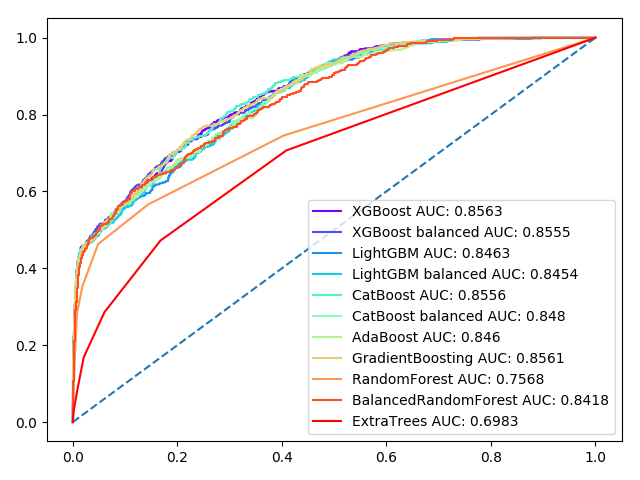
\includegraphics[width=\linewidth]{../images/roc-comparison.png}
        \caption{Porównanie krzywych ROC podstawowych modeli klasyfikacyjnych}
        \label{fig:roc-comparison}
    \end{wrapfigure}

    Warto porównać wyniki modeli XGBoost, LightGBM i CatBoost w standardowej konfiguracji z konfiguracją mająca na celu zmniejszyć problem nie zbalansowanych klas (oznaczone przez sufiks \textit{balanced}).
    Dla każdego z tych modeli, konfiguracja zbalansowana znacząco poprawiła czułość modelu, kosztem precyzji, ale pogorszyła też wartość metryki F1.
    Nie można jednak jednoznacznie stwierdzić która z tych konfiguracji jest lepsza dla omawianego zbioru danych ponieważ metryka która służy do ostatecznej ewaluacji (precyzja@10) jest niemalże identyczna w wszytkich przypadkach.

    \begin{table}
        \hspace*{-1cm}
        \begin{tabular}{l|*{6}{c}}
            & AUC & Dokładność & Precyzja@10 & F1 & Precyzja & Czułość \\
            \hline
            XGBoost & \textbf{0.8563} & \textbf{0.9516} & \textbf{0.3600} & \textbf{0.5442} & \textbf{0.7524} & 0.4262 \\
            XGBoost balanced & 0.8555 & 0.7742 & 0.3588 & 0.3043 & 0.1923 & 0.7288 \\
            LightGBM & 0.8463 & 0.9508 & 0.3575 & 0.5310 & 0.7483 & 0.4114 \\
            LightGBM balanced & 0.8454 & 0.8654 & 0.3488 & 0.3631 & 0.2672 & 0.5664 \\
            CatBoost & 0.8556 & 0.9514 & 0.3500 & 0.5418 & 0.7492 & 0.4244 \\
            CatBoost balanced & 0.8480 & 0.8450 & 0.3563 & 0.3467 & 0.2426 & 0.6070 \\
            AdaBoost & 0.8460 & 0.9505 & 0.3550 & 0.5308 & 0.7417 & 0.4133 \\
            GradientBoosting & 0.8561 & 0.9510 & 0.3588 & 0.5410 & 0.7404 & 0.4262 \\
            RandomForest & 0.7568 & 0.9404 & 0.3250 & 0.2891 & 0.7519 & 0.1790 \\
            BalancedRandomForest & 0.8418 & 0.7332 & 0.3575 & 0.2707 & 0.1661 & \textbf{0.7306} \\
            ExtraTrees & 0.6983 & 0.9328 & 0.2162 & 0.0561 & 0.5714 & 0.0295 \\
        \end{tabular}
        \hspace*{1cm}
        \caption{Metryki podstawowych modeli klasyfikacyjnych}
        \label{tab:score-comparison}
    \end{table}

    \subsection{Balansowanie klas}

    Podczas eksperymentów można było zaobserwować skłonność modeli do klasyfikowania większości obserwacji do klasy 0.
    Było to spowodowane nierównym stosunkiem liczby elementów pomiędzy klasami.
    Zbiór danych posiadał niecałe 8\% obserwacji należących do klasy 1.
    Aby rozwiązać ten problem, przeanalizowano następujące metody:
    \begin{itemize}
        \item zmniejszenie ilości obserwacji z klasy 0,
        \item zwiększenie ilości obserwacji z klasy 1,
        \item dodanie sztucznych obserwacji z klasy 1 używając techinki SMOTE~\cite{smote}.
    \end{itemize}
    Niestety, żadne rozwiązanie nie przyniosło pozytywnych rezultatów.

    \subsection{Wybór cech}
    Przygotowany zbiór danych posiadał 470 różnych kolumn.
    Aby ograniczyć ich liczbę, spróbowano wybrać te, które są najważniejsze do dokonania poprawnej klasyfikacji.
    W tym celu, po wytrenowaniu modeli XGBoost, LightGBM oraz CatBoost (w domyślnej konfiguracji oraz w konfiguracji biorącej pod uwagę balans klas), dla każdego z nich wzięto po 30 cech które okazały się najważniejsze w treningu.
    Po złączeniu tych zbiorów otrzymano nowy zbiór zawierający 57 różnych cech.
    Następnie, wszystkie wyżej wspomniane modele zostały ponownie wytrenowane na zmniejszonym zbiorze danych.
    Niestety, osiągnięte wyniki nie przyniosły żadnych pozytywnych rezultatów.

    \section{Wybrany model}

    \subsection{Dobór hiperparametrów}
    Na podstawie analizy wyników podstawowych modeli klasyfikacyjnych, zdecydowano o dokładniejszym zbadaniu modelu XGBoost.
    Aby osiągnąć wyższe rezultaty, wykorzystano metodę \textit{Grid Search} do wyszukania optymalnych parametrów.
    Wzięto pod uwagę następujące parametry modelu: stosunek klas, maksymalna głębokość drzew wchodzących w skład komitetu (base learners), współczynnik uczenia, liczbę członków komitetu oraz współczynniki próbkowania.
    Dla każdej kombinacji tych parametrów sprawdzono jakość modelu metodą kroswalidacji na 3 różnych próbach.
    Aby osiągnąć bardziej wiarygodne wyniki warto zwiększyć liczbę prób do co najmniej 5, jednak ze względu na długi czas obliczeń nie było takiej możliwości.
    Zostały wybrane te parametry, dla których model osiągnął najwyższą wartość metryki precyzja@10.

    \subsection{Kroswalidacja}
    Dla dobranych hiperparametrów została przeprowadzona ostateczna ocena jakości modelu.
    Ponownie użyto metody kroswalidacji dla 5 różnych prób.
    Wyniki modelu dla każdej próby były do siebie zbliżone.
    Dokładne wyniki są przedstawione w Tablicy~\ref{tab:xgb-score-comparison}.
    Średnia wartość metryki precyzja@10 wyniosła 40.27\%.

    %    \begin{figure}[!h]
    %        \centering
    %        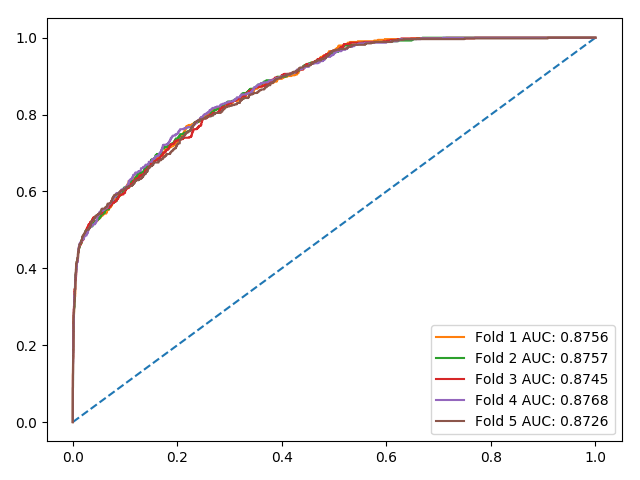
\includegraphics[width=\textwidth]{../images/xgb-roc-comparison.png}
    %        \caption{Porównanie krzywych ROC zoptymalizowanego modelu XGBoost używając kroswalidacji}
    %        \label{fig:xgb-roc-comparison}
    %    \end{figure}

    \begin{table}
        \hspace*{1cm}
        \begin{tabular}{l|*{6}{c}}
            & AUC & Dokładność & Precyzja@10 & F1 & Precyzja & Czułość \\
            \hline
            Próba 1 & 0.8605 & 0.7779 & 0.4000 & 0.3210 & 0.2071 & 0.7131 \\
            Próba 2 & 0.8757 & 0.7960 & 0.4263 & 0.3625 & 0.2395 & 0.7448 \\
            Próba 3 & 0.8702 & 0.7770 & 0.4075 & 0.3283 & 0.2099 & 0.7530 \\
            Próba 4 & 0.8621 & 0.7758 & 0.3987 & 0.3215 & 0.2055 & 0.7378 \\
            Próba 5 & 0.8569 & 0.7755 & 0.3812 & 0.3087 & 0.1971 & 0.7110 \\
            \hline
            Średnia & 0.8651 & 0.7804 & \textbf{0.4027} & 0.3284 & 0.2118 & 0.7319 \\
        \end{tabular}
        \caption{Metryki zoptymalizowanego modelu XGBoost używając kroswalidacji}
        \label{tab:xgb-score-comparison}
    \end{table}

    \section{Podsumowanie}
    Osiągnięty wynik (40.27\%) znacznie odbiega od idealnego (70\%).
    Jednakże, biorąc pod uwagę fakt silnej anonimizacji zbioru danych, jest to wynik satysfakcjonujący.
    Warto zauważyć, że wyniki zastosowanych modeli klasyfikacyjnych były do siebie zbliżone, a optymalizacja hiperparametrów dla wybranego modelu (XGBoost) przyniosła poprawę jego jakości zbliżoną do 4\%.
    Dlatego przypuszcza się że główną przeszkodą w osiągnięciu wyższej dokładności jest słaba znajomość zbioru danych i ograniczone możliwości jego analizy.

    \bibliographystyle{plain}
    \bibliography{report.bib}

    \newpage
    \begin{appendices}

        \section{Rozkład cech numerycznych z podziałem na zbiór}\label{appendix:rozklad-cech-numerycznych-zbiory}

        \begin{figure}[!h]
            \centering
            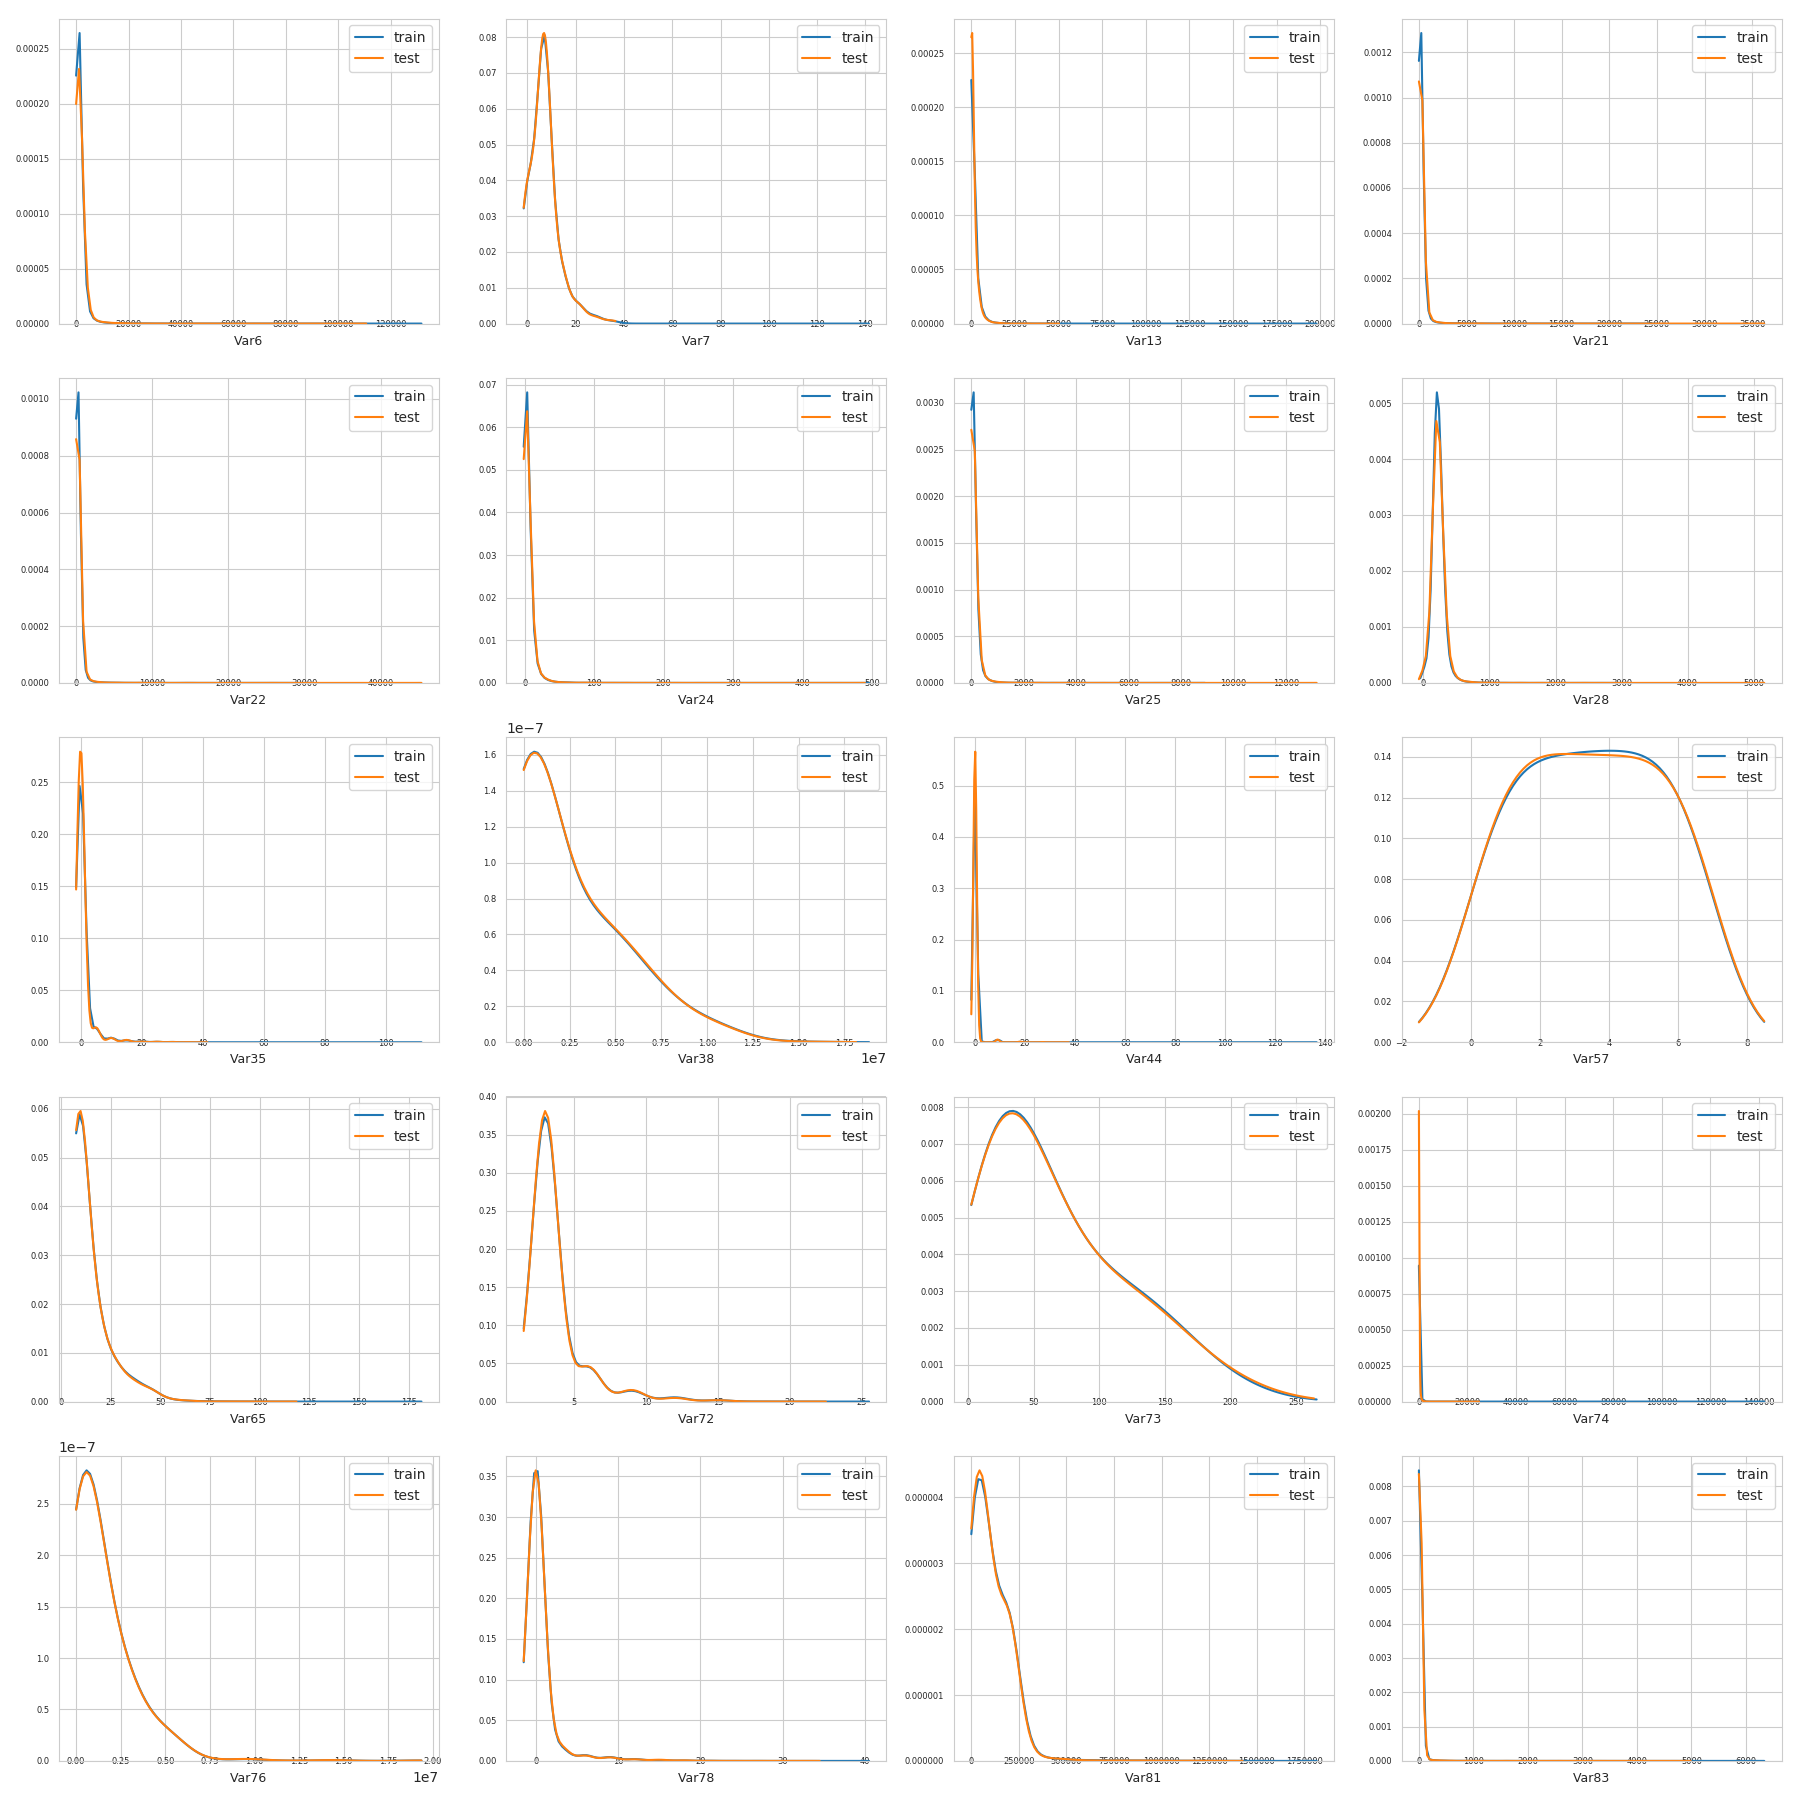
\includegraphics[width=0.9\textwidth]{../images/feature-distribution-0-20-train-test.png}
            \caption{Rozkład cech numerycznych z podziałem na zbiór}
        \end{figure}

        \newpage

        \begin{figure}[!h]
            \centering
            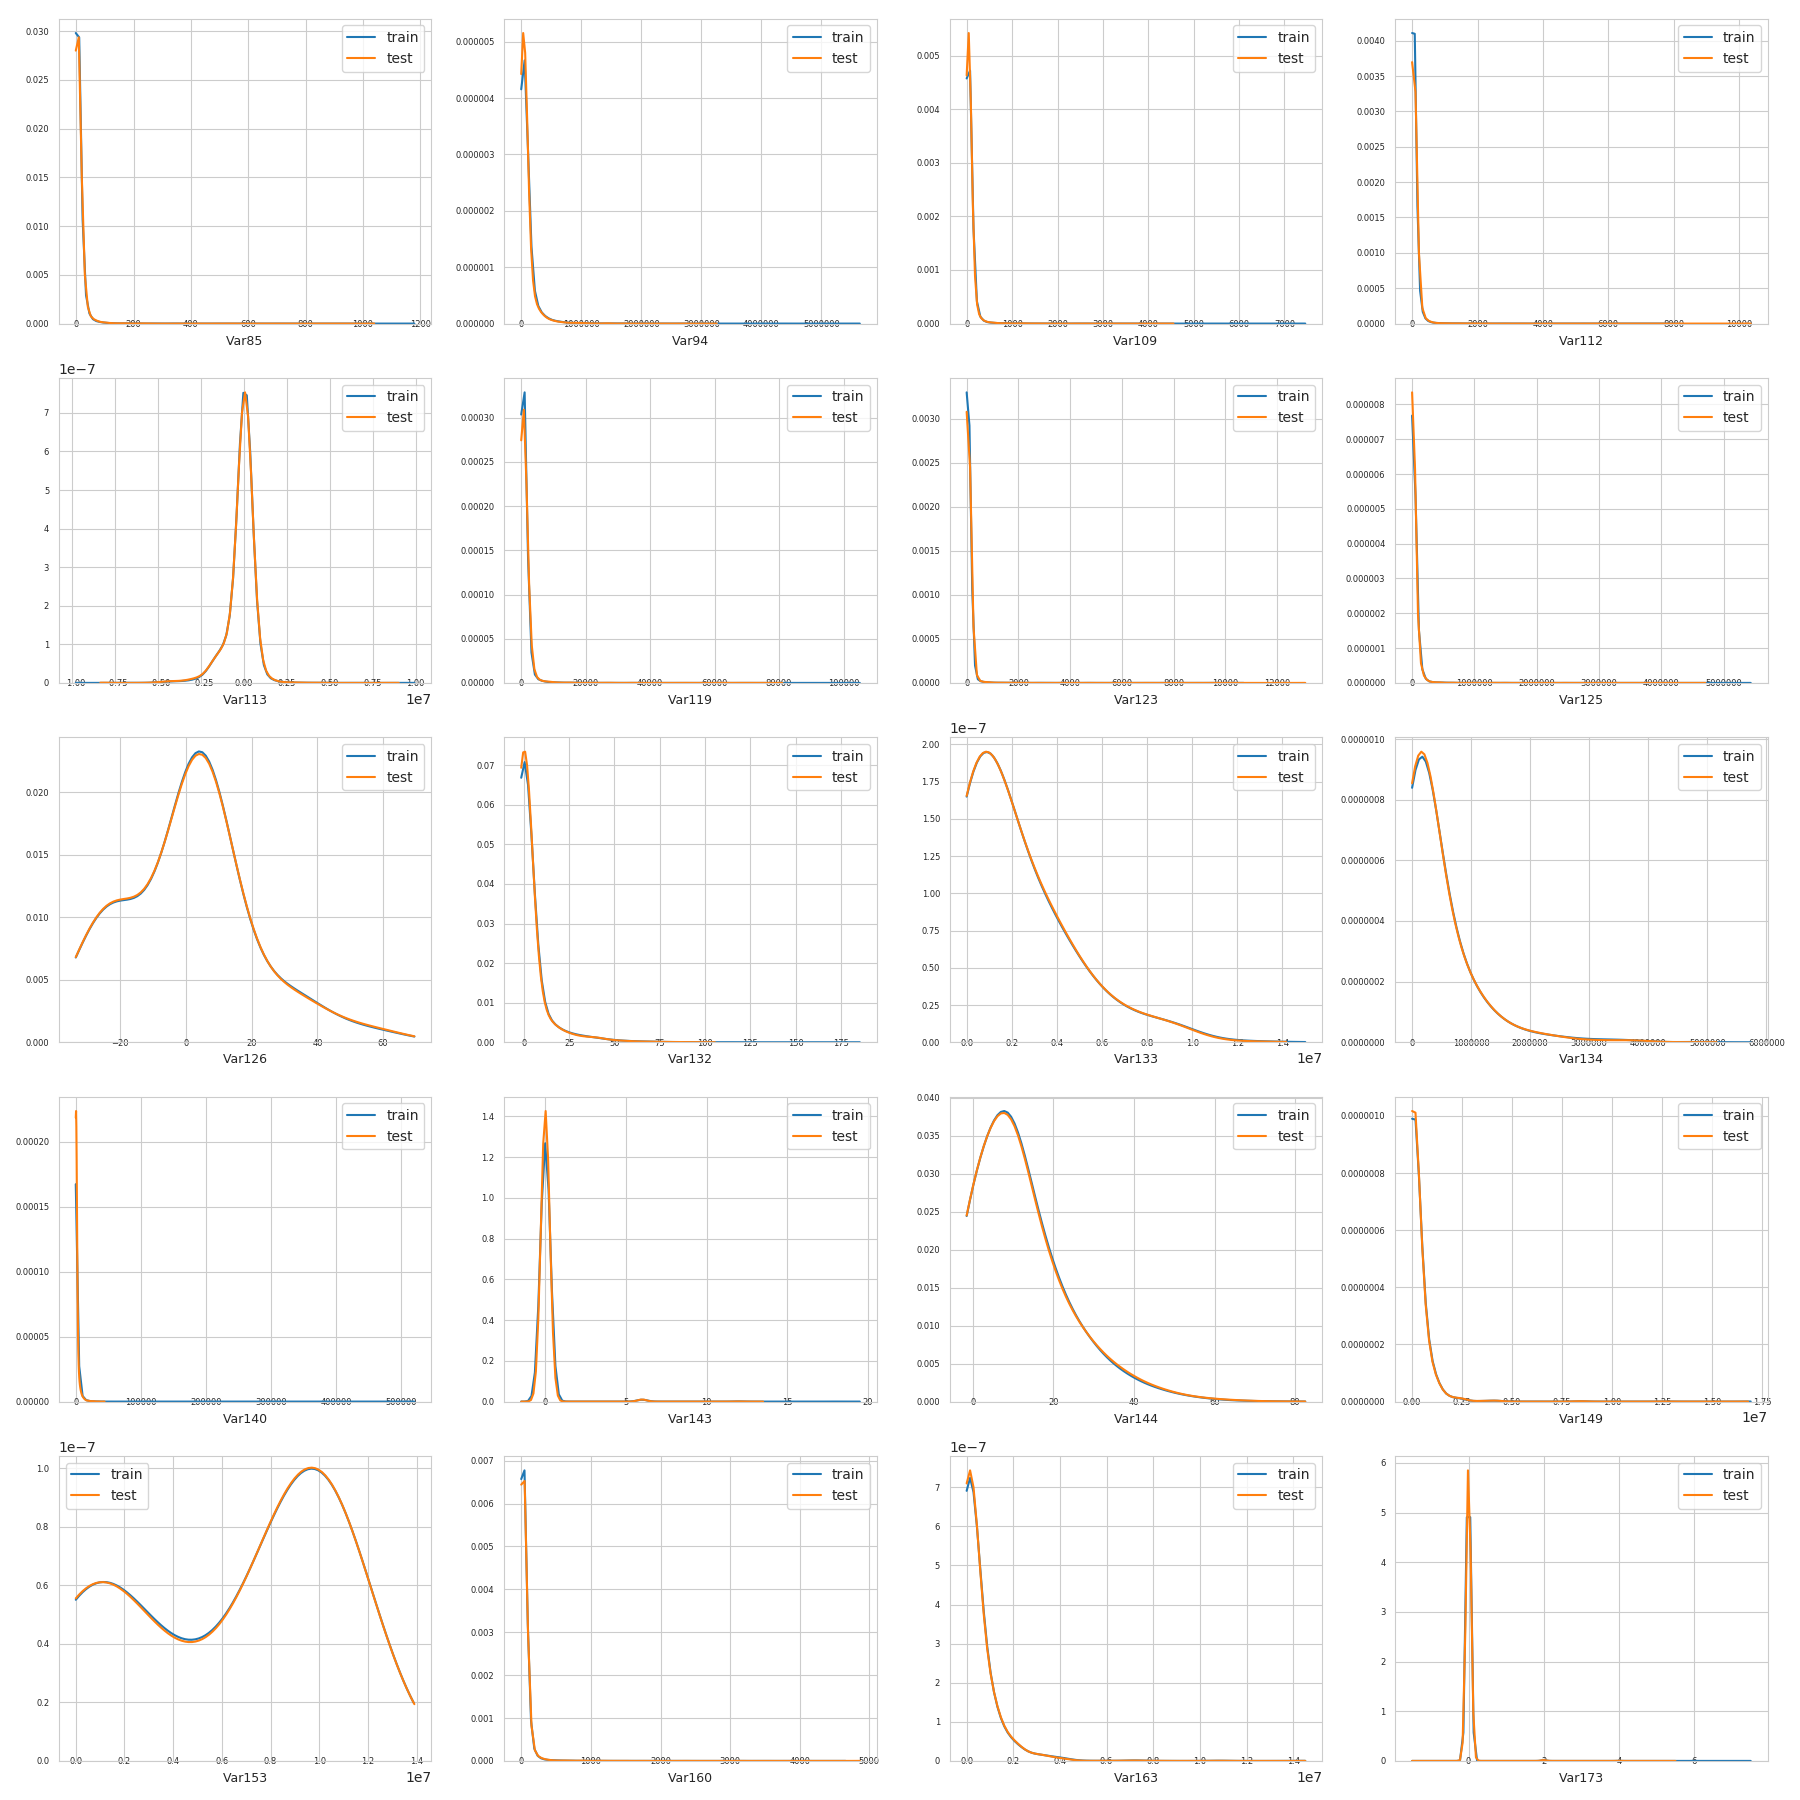
\includegraphics[width=0.9\textwidth]{../images/feature-distribution-20-40-train-test.png}
            \caption{Rozkład cech numerycznych z podziałem na zbiór}
        \end{figure}

        \newpage

        \section{Rozkład cech numerycznych z podziałem na klasę}\label{appendix:rozklad-cech-numerycznych-klasy}

        \begin{figure}[!h]
            \centering
            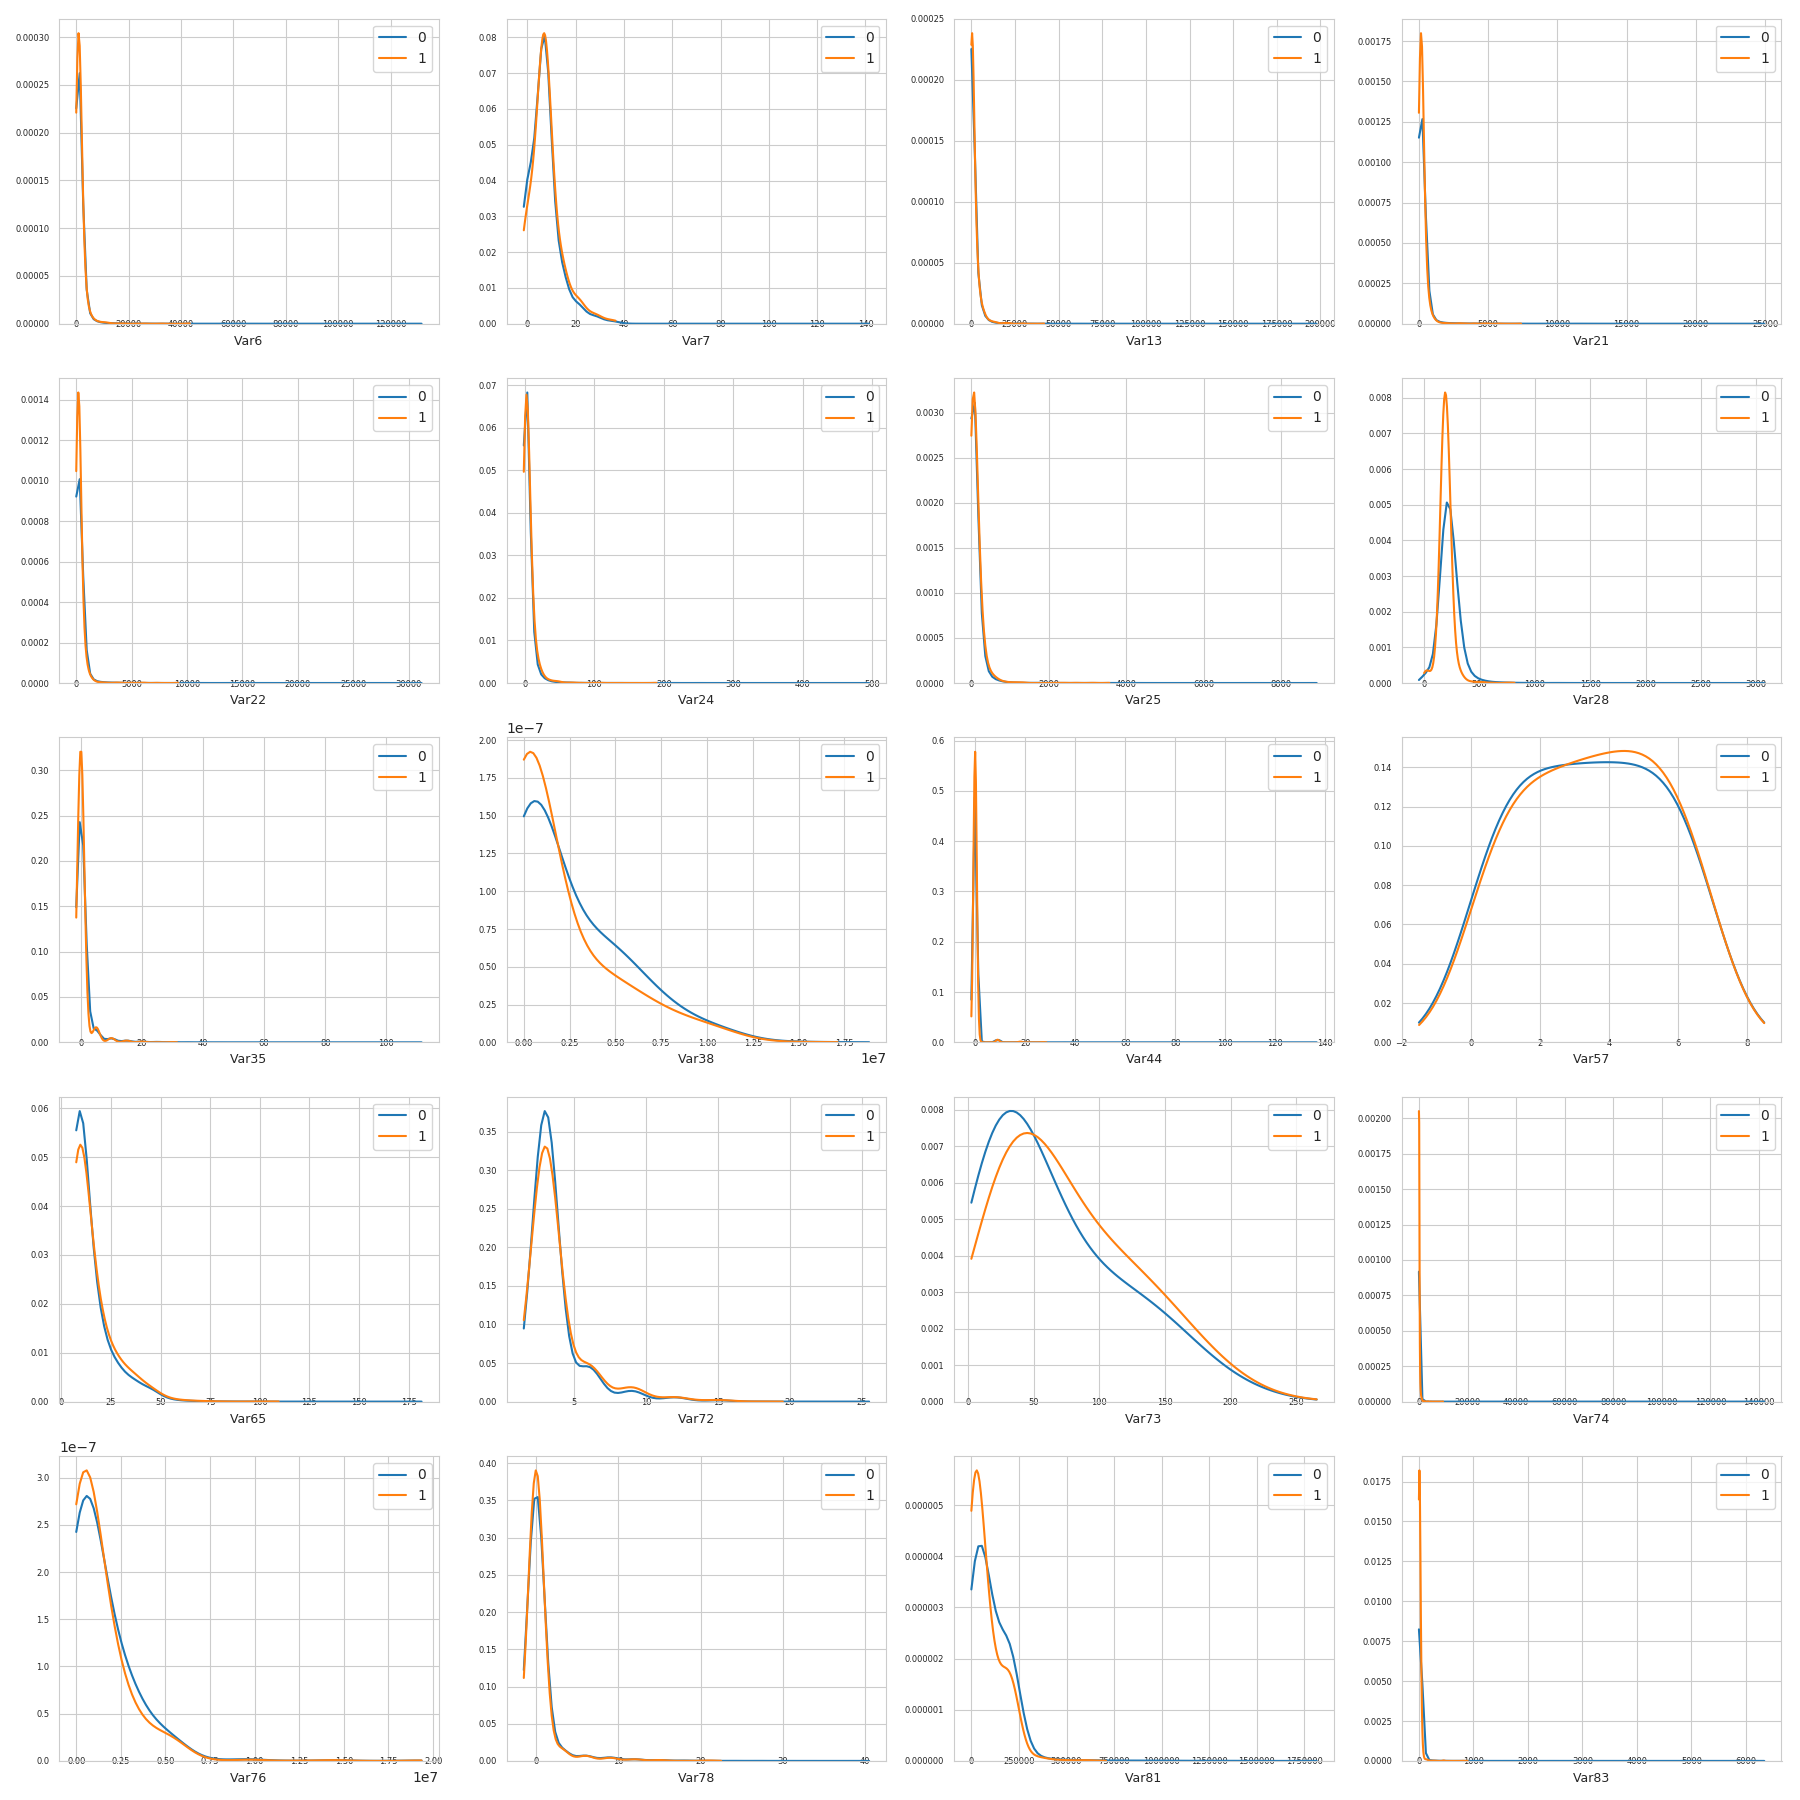
\includegraphics[width=0.9\textwidth]{../images/feature-distribution-0-20.png}
            \caption{Rozkład cech numerycznych z podziałem na klasę}
        \end{figure}

        \newpage

        \begin{figure}[!h]
            \centering
            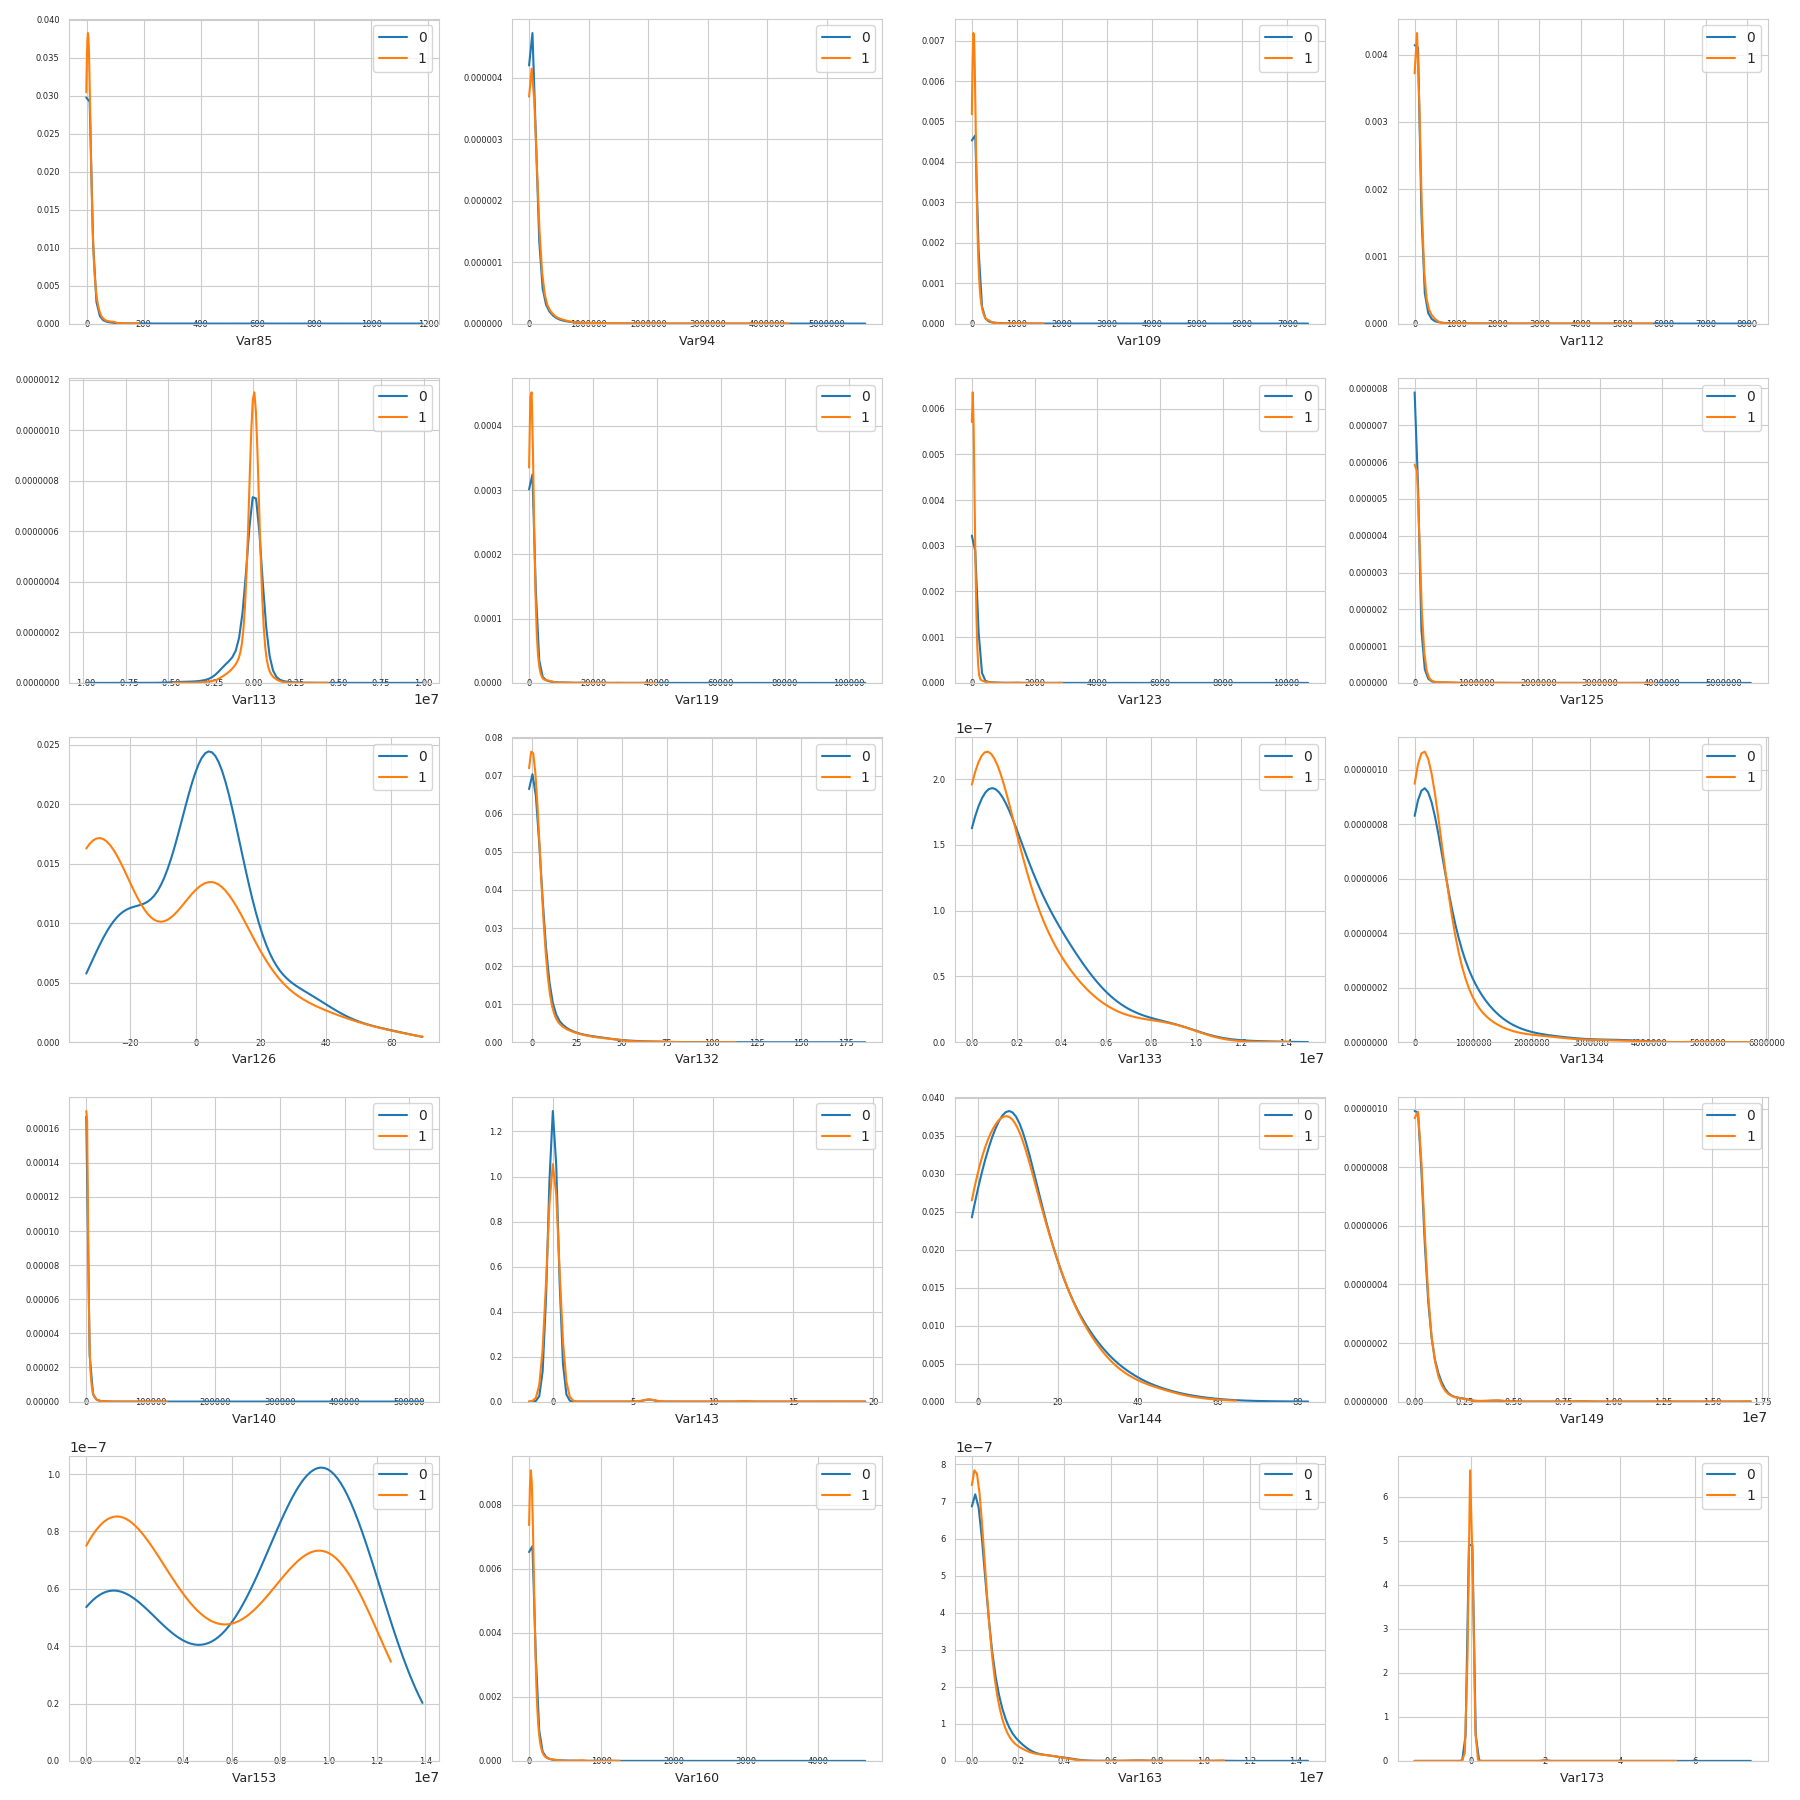
\includegraphics[width=0.9\textwidth]{../images/feature-distribution-20-40.png}
            \caption{Rozkład cech numerycznych z podziałem na klasę}
        \end{figure}

    \end{appendices}

\end{document}
